%!TEX root = ../main.tex
\vspace*{\fill}

{\large \bf Chapter~\ref{chp:slp_ortho} Authorship Statement}

\vspace{1em}

{\bf Citation:} Pierre-Olivier Goffard, Patrick J.\ Laub (2017), \emph{Two numerical methods to evaluate stop-loss premiums}, Scandinavian Actuarial Journal (submitted)

\vspace{1em}

The authors of this paper equally contributed to the following tasks:
\begin{enumerate}
\item conception and design of the project;
\item mathematical arguments, and interpretation of the results;
\item writing the publication.
\end{enumerate}

In addition to this, I completed the majority of the computational work and of the editing (e.g.\ checking grammar and typographical details).

\vspace{3em}

\vspace*{\fill}

\chapter{Two numerical methods to evaluate stop-loss premiums} \label{chp:slp_ortho}
\section{Introduction}\label{sec:Introduction}

Consider the random variable
\begin{equation*}\label{eq:AggregatedClaimAmountsRV}
S_N=\sum_{k=1}^{N}U_{k},
\end{equation*}
where $N$ is a counting random variable and $\{U_{k}\}_{k\in\NZ}$ is a sequence of random variables which are iid, non-negative, and independent of $N$.
We denote the pdf of $S_N$ as $f_{S_N}$, and its survival function as
\begin{equation*}\label{eq:DefinitionSurvivalFunction}
\Ftail_{S_N}(x)= \Prob(S_N>x),\quad \text{ for } x\geq0.
\end{equation*}
This chapter concerns approximations of $f_{S_N}$ and $\Ftail_{S_N}$ though we begin with a discussion of how $S_N$ is used in actuarial science.

Frequently $S_N$ models the aggregated losses of a non-life insurance portfolio over a given period of time---here $N$ represents the number of claims and $U_k$ the claim sizes---yet other applications also exist. Actuaries and risk managers typically want to quantify the risk of large losses by a single comprehensible number, a risk measure.

One popular risk measure is the VaR. In actuarial contexts, the VaR at level $\alpha \in (0,1)$ is defined such that the probability of (aggregated) losses exceeding the level VaR is at most $1-\alpha$.
Following the European recommendation of the Solvency II directive, the standard value for $\alpha$ is $0.995$, see \cite{EIOPA}. It is used by risk managers in banks, insurance companies, and other financial institutions to allocate risk reserves and to determine solvency margins. Also, we have stop-loss premiums which are risk measures that are commonly used in reinsurance agreements.

A reinsurance agreement is a common risk management contract between insurance companies, one called the \emph{cedant} and the other the \emph{reinsurer}. Its aim is to keep the cedant's long-term earnings stable by protecting the cedant against large losses. The reinsurer absorbs part of the cedant's loss, say $f(S_N)$ where $0\leq f(S_N)\leq S_N$, leaving the cedant with $I_{f}(S_N)=S_N-f(S_N)$. In return, the cedant pays a premium linked to
\begin{equation*}\label{eq:DefinitionReinsurancePremium}
\Pi=\Exp[f(S_N)],
\end{equation*}
under the expected value premium principle.


In practice, there are a variety of reinsurance designs from which an insurer can choose. We focus in this work on the stop-loss reinsurance treaty associated with the following ceded loss function
\begin{equation*}\label{eq:StopLossCededFunction}
f(S_N)=(S_N-a)_{+},\text{ }a\geq0,
\end{equation*}
where $a$ is referred to as the retention level or priority. The ratemaking of the stop-loss reinsurance policy requires the evaluation of
\begin{equation}\label{eq:DefUsualStopLossPremium}
\Pi_{a}(S_N)=\Exp\left[(S_N-a)_{+}\right],
\end{equation}
also known as the usual stop loss premium.

One variation is the limited stop-loss function,
\begin{equation}\label{eq:LimitedStopLossCededFunction}
f(S_N)=\min[(S_N-a)_{+},b],\text{ }b\geq0,
\end{equation}
where $b$ is called the limit. The limited stop-loss function \eqref{eq:LimitedStopLossCededFunction} is very appealing in practice because it prevents the cedant from over-estimating their losses and therefore over-charging the reinsurer.
Also, the change-loss function is defined as
\begin{equation*}\label{eq:ChangeLossCededFunction}
f(S_N)=c(S_N-a)_{+},\text{ }0\leq c\leq1,
\end{equation*}
which is in between stop-loss and quota-share reinsurance. The ratemaking in each case requires the expectation in \eqref{eq:DefUsualStopLossPremium}.

From a practical point of view, a reinsurance treaty over the whole portfolio is less expensive to handle than one which involves claim-by-claim management. It also grants protection in the event of an unusual number of claims, triggered for instance by a natural disaster. From a theoretical point of view, it is well known that the stop-loss ceded function allows one to minimise the variance of the retained loss for a given premium level, see for instance the monograph of Denuit et al.\ \cite{DeDhGoKa06}. Recently, it has been shown that stop-loss reinsurance is also optimal when trying to minimise the VaR and the expected shortfall of the retained loss, see the works of Cai et al.\ \cite{CaTaWeZh08}, Cheung \cite{Ch10}, and Chi and Tan \cite{ChTa11}. Note that some other ceded loss functions appear in their work, there are however very close to the stop-loss one.

Unfortunately, one is seriously constrained when calculating these quantities analytically, as there are only a few cases where either the pdf or the survival function is available in a simple tractable form. To estimate the VaR or the stop-loss premium we must find fast and accurate approximations for these functions.

We discuss the use of an approximation of the pdf in terms of the gamma density and its orthonormal polynomials. This method has been studied in the recent works of Goffard et al.\ \cite{GoLoPo15} and Jin et al.\ \cite{JiPrRe16}. We emphasise here the computational aspect of this numerical method and detail some practical improvements. An exponential change of measure can be used to recover the pdf of $S_N$ when the claim sizes are governed by a heavy-tailed distribution. This refinement has been successfully applied in Chapter~\ref{chp:sln_orth_pdf} to recover the density of the sum of lognormally distributed random variables.

This method is compared to a numerical inversion of the Laplace transform which is known to be efficient to recover the survival function of a compound distribution. The critical step in Laplace inversion is to select which numerical integration technique to apply. We implement a method inspired by the work of Abate and Whitt \cite{Abate1992} which is very similar to the method of Rolski et al.\ \cite[Chapter 5, Section 5]{RoScScTe08}. An approximation of the stop-loss premium is then proposed relying on the connection with the survival function of the equilibrium distribution of $S_N$. Note that Dufresne et al.\ \cite{DuGaMo09} successfully applied a Laplace inversion based technique to the evaluation of stop-loss premiums.

To close, we want to emphasise the fact that the numerical methods also apply in a risk theory framework. The infinite-time ruin probability in the compound Poisson ruin model is equal to the survival function of a compound geometric distribution. The polynomial approximation and the Laplace inversion methods have been employed, and compared to solve this particular problem in the work of Goffard et al.\ \cite{GoLoPo16}. We add a more original application by noting that the finite-time non-ruin probability with no initial reserves, again under the classical risk model assumptions, may be rewritten as the stop-loss premium associated with a compound Poisson distribution where the priority is expressed in terms of the premium rate and the time horizon.

The rest of the chapter is organised as follows. Section \ref{sec:Preliminaries} introduces compound distributions, and details their role in risk theory. Section \ref{sec:PolynomialApproximation} presents the approximation method based on orthogonal polynomials. Section \ref{sec:NumericalInversionLaplaceTransform} presents the approximation through the numerical inversion of the Laplace transform. Section \ref{sec:NumericalIllustrations} is devoted to numerical illustrations where the performances of the two methods are compared; the \textsc{Mathematica} code used is available online \cite{StoplossCode}.

\section{Compound distributions and risk theory}\label{sec:Preliminaries}

We introduce compound distributions along with a brief account of their importance in risk modeling.

\subsection{Compound distributions}

Let $S_N=\sum_{k=1}^{N}U_k$ be the aggregated claim amounts associated with a non-life insurance portfolio over a fixed time period. The number of claims, also called the claim frequency, is modeled by a counting random variable $N$ having a probability mass function $f_N$. The claim sizes form a sequence $\{U_k\}_{k\in \NZ}$ of iid non-negative random variables with common pdf $f_{U}$. We further assume that the claim sizes are independent from the claim frequency.

As $S_N=0$ whenever $N=0$ (assuming this occurs with positive probability), the distribution of $S_N$ is the sum of a singular part (the probability mass $\Prob(S_N=0)=f_N(0)>0$) and a continuous part (describing $S_N$ where $N>0$) with a defective pdf $f_{S_N}^+$ and cdf $F_{S_N}^+$. From the law of total probability, we have
\begin{equation}\label{eq:DefectivePDFCompoundDistribution}
f_{S_N}^+(x)=\sum_{n=1}^{\infty}f_N(n)f_{U}^{\ast n}(x),~x\geq0.
\end{equation}

This density is intractable because of the infinite series. Furthermore, the summands are defined by repeated convolution of $f_{U}$ with itself which are rarely straightforward to evaluate. The methods presented in this work rely on the knowledge of the Laplace transform of $S_N$, given by
\begin{equation*}\label{eq:TransformsForCompoundDistribution}
\LTsub{S_N}(t) = \PGF_N[ \LTsub{U}(t) ] \,,
\end{equation*}
where $\PGF_N(t) \defeq \Exp[t^N]$ is the \emph{probability generating function} of $N$. The simple expression of the Laplace transform has made possible the use of numerical methods involving the moments or transform inversion to recover the distribution of $S_N$. The distribution is typically recovered using Panjer's algorithm or a Fast Fourier Transform algorithm based on the inversion of the discrete Fourier transform; these two methods are compared in the work of Embrechts and Frei \cite{embrechts2009panjer}. Our orthogonal polynomial method involves the standard integer moment sequence for $S_N$, in contrast to more exotic types of moments used by some recent methods. Gzyl and Tagliani \cite{GzTa12} uses the fractional moments within a max-entropic based method, while Mnatsakanov and Sarkisian \cite{Mnatsakanov2013} performs an inversion of the scaled Laplace transform via the exponential moments. In addition to proposing an approximation for the survival function of $S_N$, we provide an efficient way to compute the usual stop-loss premium \eqref{eq:DefUsualStopLossPremium} for reinsurance applications.

\subsection{Risk theory}

In the classical risk model, the financial reserves of a non-life insurance company are modeled by the risk reserve process $\{R(t),t\geq0\}$, defined as
\begin{equation*}\label{eq:RiskReserveProcess}
R(t)=u+ct-\sum_{k=1}^{N(t)}U_k.
\end{equation*}
The insurance company holds an initial capital of amount $R(0)=u\geq0$, and collects premiums at a constant rate of $c>0$ per unit of time. The number of claims up to time $t\geq0$ is governed by a homogeneous Poisson process $\{N(t),t\geq0\}$ with intensity $\lambda$. The claim sizes are iid non-negative random variables independent from $N(t)$.

One of the goals of risk theory to evaluate an insurer's ruin probability, that is, the probability that the financial reserves eventually fall below zero. Of interest are both the finite-time ruin probability $\psi(u,T)$ and the infinite-time ruin probability, also called the \emph{probability of ultimate ruin}, $\psi(u)$, which are defined as
\begin{equation*}\label{eq:FiniteTimeRuinProbability}
\psi(u,T)=\Prob\Bigl( \inf_{0 \le t \le T} R(t) \leq 0 \Bigr)\,,
\end{equation*}
and
\begin{equation*}\label{eq:InfiniteTimeRuinProbability}
\psi(u)=\Prob\Bigl( \inf_{t \geq 0}\,R(t) \leq 0 \Bigr)\,.
\end{equation*}
These probabilities are often reformulated (for mathematical convenience) in terms of the associated claims surplus process $\{S(t),t\geq0\}$,
\begin{equation*} \label{eq:ClaimsSurplusProcess}
S(t) = \sum_{k=1}^{N(t)} U_k - ct,\text{ }t\geq0,
\end{equation*}
specifically,
\begin{equation*}
\psi(u,T)=\Prob\Bigl( \sup_{0 \le t \le T} S(t) \geq u \Bigr) \quad \text{and} \quad
\psi(u)=\Prob\Bigl( \sup_{t \geq 0}\,S(t) \geq u \Bigr).
\end{equation*}

For a general background on risk theory and the evaluation of ruin probabilities, we refer the reader to the monograph of Asmussen and Albrecher \cite{asmussen2010ruin}.

The first connection between compound distributions and ruin probabilities is the following.
If the net benefit condition is satisfied, i.e.\ if the premium rate exceeds the average cost of aggregated claims per unit of time, then the infinite-time ruin probability is given by the survival function of a geometric compound distribution. More precisely,
\begin{equation*}\label{eq:PollaczeckKhinchineFormula}
\psi(u) = \Prob\Bigl(S_N \defeq \sum_{k=1}^{N}U^\ast_{k}>u\Bigr)
= (1 - \rho) \sum_{n=1}^\infty \rho^n \Ftail_{U^\ast}^{\ast n}(u),
\end{equation*}
with $N \sim \mathsf{Geom}_0(\rho)$, $\rho = \lambda\Exp[U]/c<1$, and with iid $U^\ast_{k}$ with pdf $f_{U^\ast}(x)= \Ftail_U(x) / \Exp[U]$. This result is known as the Pollaczeck--Khinchine formula, see for instance Asmussen and Albrecher \cite[Chapter IV, (2.2)]{asmussen2010ruin}. Thus it is possible to evaluate the infinite-time ruin probability via Panjer's algorithm. If we are able to determine the Laplace transform of $V$ then we can also apply the polynomial method of Goffard et al.\ \cite{GoLoPo15}, the fractional moment based method of Gzyl et al.\ \cite{GzNITa13}, and the exponential moments based method of Mnatsakanov et al.\ \cite{Mnatsakanov2015}.

The second connection links the finite-time ruin probability with no initial reserves to the stop-loss premium associated with a compound distribution.
If $N(t) \sim \mathsf{Poisson}(\lambda t)$ (i.e.\ claims arrive as a homogeneous Poisson process) then the finite-time ruin probability is given by
\begin{align} \label{CramersFormula}
\psi(0, T)
&= 1 - \frac{1}{cT} \int_0^{cT} \Prob \Bigl( \, \sum_{i=1}^{N(T)} U_i \le x \Bigr) \dd x \,.
\end{align}
This implies $\psi(0,T) = \Exp [ \min( S_{N(T)}, cT ) ]/cT$ where $S_{N(T)} \defeq \sum_{i=1}^{N(T)} U_i$, and hence
\begin{align} \label{eq:ConnectionFiniteTimeRuinProbabilityStopLossPremium}
\psi(0, T)
&= \frac{1}{cT} \Exp[ \min( S_{N(T)}, cT ) ] \nonumber \\
&= (cT)^{-1} \{ \Exp[N(T)] \, \Exp[U_1] - \Pi_{cT}(S_{N(T)}) \} \,.
\end{align}
Lef\`evre and Picard \cite[Corollary~4.3]{LePi11} show that equations \eqref{CramersFormula} and \eqref{eq:ConnectionFiniteTimeRuinProbabilityStopLossPremium} hold in the more general case where the claim arrival process forms a \textit{mixed Poisson process}. This connection has been exploited recently in Lef\`evre et al.\ \cite{LeTrZu17} where the influence of the claim size distribution on the ruin probabilities is studied via stochastic ordering considerations.

\section{Orthogonal polynomial approximations}\label{sec:PolynomialApproximation}


\subsection{Approximating general density functions} \label{ssec:PolynomialApproxIntro}

Let $X$ be an arbitrary random variable with pdf $f_X$.\footnote{This section is written from the perspective of approximating a pdf, however the main results also hold if applied to a defective density.} We assume that the density is unknown and we propose an approximation of the form
\begin{equation}\label{eq:PolynomialApproximation}
\widehat{f}_{X}(x)=\sum_{k=0}^{K}a_{k}p_{k}(x)w(x).
\end{equation}
where $w$ is the \emph{reference density}. The $\{p_{k}\}_{k\in\NZ}$ are the polynomials which are orthonormal with respect to $w$, just as in Chapters~\ref{chp:intro} and \ref{chp:sln_orth_pdf}.

Just as earlier, we can generate the polynomials by the Gram--Schmidt procedure if $w$ admits moments of all orders (i.e.\ $\forall n \in \NZ :$ $\Exp[X^n] < \infty$ where $X \sim w$), and the resulting polynomials are complete in $\Lp^2(\RL, w(x) \dd x)$ if $\int_{\RL} \e^{s\abs{x}} w(x) \dd x < \infty$ for some $s>0$.

Therefore, if $f_{X}/w\in \Lp^2(\RL, w(x) \dd x)$ we have
\begin{equation}\label{eq:PolynomialRepresentationTheory}
f_{X}(x)/w(x)=\sum_{k=0}^{\infty} \langle f_X / w, p_k \rangle_w p_k(x) \,.
\end{equation}
We label the coefficients as $a_k = \langle f_X / w, p_k \rangle_w = \Exp[p_k(X)]$
and rearrange \eqref{eq:PolynomialRepresentationTheory} to be
\begin{equation}\label{eq:PolynomialRepresentation}
f_{X}(x)=\sum_{k=0}^{\infty} a_k p_{k}(x) w(x).
\end{equation}
The approximation \eqref{eq:PolynomialApproximation} follows by simply truncating the series to $K+1$ terms.

Typical choices of reference distributions are ones that belong to a Natural Exponential Family with Quadratic Variance Function (NEF-QVF) which includes the normal, gamma, hyperbolic, Poisson, binomial, and Pascal distributions.
This family of distributions is convenient as the associated orthogonal polynomials are classical, see the characterisation by Morris \cite{Mo82}. The polynomials are known explicitly, so the time-consuming Gram--Schmidt orthogonalisation procedure is unneccessary. Furthermore, it has been shown in a paper by Provost \cite{Pr05} that the recovery of unknown densities from the knowledge of the moments of the distribution naturally leads to an approximation in terms of the gamma density and Laguerre polynomials when $X$ admits $\RL_{+}$ as support, and in terms of the normal density and Hermite polynomials when $X$ has $\RL$ as support.

\subsection{Approximating densities of positive random variables} \label{ssec:PolynomialApproxPositive}

To approximate the pdf for positive $X$, a natural candidate for the reference density is the gamma density. It has been proven to be efficient in practice, see the work of Goffard et al.\ \cite{GoLoPo15,GoLoPo16}, and Jin et al.\ \cite{JiPrRe16}. The work of Papush et al.\ \cite{PaPaPo01} showed that among the gamma, normal and lognormal distributions, the gamma distribution seems to be better suited to model certain aggregate losses. The lognormal distribution is a problematic choice. Even though the orthogonal polynomials are available in a closed form (see Section~\ref{app:lognormal_poly}), Proposition~\ref{prop:ln_incomplete} shows that they are incomplete in $\Lp^2(\RL, w(x) \dd x)$. The case of the inverse Gaussian as basis received a treatment in the work of Nishii \cite{Ni96}, where it is shown that the only way to get a complete system of polynomials is by using the Gram--Schmidt orthogonalisation procedure. Differentiating the density (as it is done in the case of NEF-QVF) does not lead to an orthogonal polynomial system, and starting from the Laguerre polynomials leads to a system of orthogonal functions which is not complete. A solution might be to exploit the bi-orthogonality property pointed out in the work of Hassairi and Zarai \cite{HaZa04}. To close this review of reference densities, we mention the work of Nadarajah et al.\ \cite{NaChJi16} where Weibull and exponentiated exponential distributions are considered as reference density.

Consider $w$ to be the pdf of the $\mathsf{Gamma}(r,m)$ distribution
and the associated orthonormal polynomials are given by
\begin{equation*}\label{eq:GeneralizedLaguerrePolynomials}
p_{n}(x)
=(-1)^{n} \binom{n + r - 1}{n}^{-\frac12} L_{n}^{r-1}\big(\frac{x}{m}\big)
=(-1)^{n} \left( \frac{\Gamma(n+r)}{\Gamma(n+1)\Gamma(r)} \right)^{-\frac12} L_{n}^{r-1}\big(\frac{x}{m}\big),
\end{equation*}
where $\{L_{n}^{r-1}\}_{n\in\NZ}$ are the generalised Laguerre polynomials,
\begin{equation*}\label{eq:GeneralizedLaguerrePolynomialsExpression}
L_{n}^{r-1}(x)
=\sum_{i=0}^{n} \binom{n + r - 1}{n - i} \frac{(-x)^i}{i!}
=\sum_{i=0}^{n} \frac{\Gamma(n+r)}{\Gamma(n-i+1)\Gamma(r+i)}\frac{(-x)^i}{i!}, \text{ }n\geq 0,
\end{equation*}
cf.\ the classical book by Szeg{\"o} \cite{Szegoe1939}.

\begin{lemma}\label{Lemma:PseudoMixtureOfGammas}
If $w$ is the pdf of the $\GammaDist(r,m)$ distribution, the polynomial expansion \eqref{eq:PolynomialRepresentation}  may be rewritten as
\begin{align}\label{eq:PseudoMixtureOfGammas}
f_{X}(x)&= \sum_{i=0}^{\infty} c_i \gamma(r+i,m,x) \,,
\end{align}
where
\begin{equation}\label{eq:PiExpression}
c_i
=\sum_{k=i}^\infty a_k \frac{(-1)^{i+k}}{i! \, (k-i)!} \sqrt{\frac{k! \Gamma(k+r)}{\Gamma(r)}},
\end{equation}
and the function $\gamma(r,m,x)$ is the pdf of the $\GammaDist(r,m)$ distribution.
\end{lemma}
\begin{proof}
If we change the sum in \eqref{eq:PolynomialRepresentation} from iterating over Laguerre polynomials to iterating over monomials we get
\[
f_{X}(x)=\sum_{k=0}^{\infty} a_k p_{k}(x) \gamma(r,m,x) = \sum_{i=0}^\infty b_i x^i \gamma(r,m,x) \,,
\]
where
\begin{align*}
b_i
&= \sum_{k=0}^\infty \text{Coefficient}(x^i, a_k  p_k(x))
= \frac{(-1)^i}{m^i i!} \sum_{k=i}^\infty a_k (-1)^{k} \binom{k + r - 1}{k}^{-\frac12} \binom{k + r - 1}{k - i} \,.
\end{align*}
We also note that
\[ x^i \gamma(r, m, x) = m^i \frac{\Gamma(r+i)}{\Gamma(r)} \gamma(r+i, m, x), \]
so
\[ f_{X}(x) = \sum_{i=0}^\infty b_i m^i \frac{\Gamma(r+i)}{\Gamma(r)} \gamma(r+i, m, x) =  \sum_{i=0}^\infty c_i \gamma(r+i, m, x),  \]
where we have set $c_i = b_i m^i \Gamma(r+i) / \Gamma(r)$.
\end{proof}

\begin{remark}
When $r=1$ (that is, when $w(x)$ is the pdf of an exponential distribution) the formula for $c_i$, \eqref{eq:PiExpression}, simplifies to
\[ c_i = \sum_{k=i}^\infty a_k (-1)^{i+k} \binom{k}{i} \,. \]
\remQED
\end{remark}

The expression of the pdf in \eqref{eq:PseudoMixtureOfGammas} resembles the one of an Erlang mixture, which are extensively used for risk modeling purposes, cf.\ Willmot and Woo \cite{WiWo07}, Lee and Lin \cite{LeLi10}, and Willmot and Lin \cite{WiLi11}. However, the $c_i$ defined in \eqref{eq:PiExpression} do not form a proper probability mass function as they are not always positive. Hence our approximation cannot be considered as an approximation through an Erlang mixture although it enjoys the same features when it comes to approximating the survival function and the stop-loss premium as shown in the following result.
\begin{proposition} \label{prop:OrthogonalPolynomialForm}
Letting $\Gamma_u(r,m,x)$ be the survival function of the $\GammaDist(r,m)$ distribution,  we have:
\begin{itemize}
\item[(i)] the survival function of $X$ is given by
\begin{equation}\label{eq:TailFunctionX}
\Ftail_{X}(x) = \sum_{i=0}^{\infty}c_i\Gamma_{u}(r+i,m,x) \quad \text{for } x \ge 0 \,,
\end{equation}
\item[(ii)] the usual stop-loss premium of $X$ with priority $a \ge 0$ is given by
\begin{equation}
\Exp\left[\left(X-a\right)_{+}\right] = \sum_{i=0}^{\infty}c_i\left[m (r+i) \Gamma_{u}(r+i+1,m,a)-a\Gamma_{u}(r+i,m,a)\right]. \label{eq:UsualStoplossX}
\end{equation}
\end{itemize}
\end{proposition}
\begin{proof}
If $f_{X}/w\in \Lp^2(\RL, w(x) \dd x)$ then Lemma~\ref{Lemma:PseudoMixtureOfGammas} allows us to write $f_X$ as in \eqref{eq:PseudoMixtureOfGammas}, and integrating this over $\left[x,\infty\right)$ yields the formula \eqref{eq:TailFunctionX}.
Now consider the usual stop-loss premium of $X$, and note that
\begin{align}
\Exp\left[(X-a)_+\right]=&\int_{a}^{\infty}(x-a)f_{X}(x)\dd x \nonumber\\
=&\int_{a}^{\infty}xf_{X}(x)\dd x-a\Ftail_{X}(a).\label{eq:UsualStopLossXProof1}
\end{align}
Then notice that for every $i \in \NL$, we have that
\begin{align}
\int_{a}^{\infty} x \, \gamma(r+i, m, x)\dd x
&= \int_{a}^{\infty}x\frac{x^{r+i-1} \e^{-x/m}}{\Gamma(r+i)m^{r+i}}\dd x\nonumber\\
&= m\frac{\Gamma(r+i+1)}{\Gamma(r+i)}\int_{a}^{\infty}\frac{x^{r+i} \e^{-x/m}}{\Gamma(r+i+1)m^{r+i+1}}\dd x\nonumber\\
&= m (r+i) \Gamma_{u}(r+i+1,m,a).\label{eq:UsualStopLossXProof2}
\end{align}
Therefore substituting \eqref{eq:PseudoMixtureOfGammas} and \eqref{eq:TailFunctionX} into \eqref{eq:UsualStopLossXProof1} and simplifying with \eqref{eq:UsualStopLossXProof2} yields \eqref{eq:UsualStoplossX}.
\end{proof}

Let us make the connection between our approach and Erlang mixture more precise. Assuming that $f_{X}/w\in\Lp^2(\RL, w(x) \dd x)$ then taking the Laplace transform on both side of \eqref{eq:PseudoMixtureOfGammas} yields
\begin{equation*}
\LTsub{X}(s)=\sum_{i=0}^{\infty} c_i \left(\frac{1}{1+sm}\right)^{r+i}
=\left(\frac{1}{1+sm}\right)^{r}\mathcal{P}\left(\frac{1}{1+sm}\right),\label{eq:PseudoErlangMixtureLaplaceTransform}
\end{equation*}
where $\mathcal{P}(z)=\sum_{i=1}^{\infty}c_i z^{i}$ denotes the generating function of the $\{c_i\}_{i\in\NZ}$ coefficients. Now setting $z=\frac{1}{1+sm}$ allows to express the generating function $\mathcal{P}(z)$ in terms of the Laplace transform of $X$ as
\begin{equation*}\label{eq:GeneratingFunctionPi}
\mathcal{P}(z)=z^{-r}\LTsub{X}\left(\frac{1-z}{zm}\right).
\end{equation*}

\begin{remark}
The approximation through an Erlang mixture consists in approximating the pdf of a nonnegative random variable $X$ as
\begin{equation*}\label{eq:ErlangMixtureRepresentation}
f_X(x)=\sum_{i=1}^{\infty}c_i\gamma(i,m,x),\text{ for }x\geq0.
\end{equation*}
The function $\mathcal{P}(z)$ becomes then the probability generating function (pgf) of a counting random variable $M$, where $c_i=\Prob(M=i),\text{ for }i\geq1$.
\remQED
\end{remark}
The next example is designed to shed light on the link between our polynomial expansion and an Erlang mixture.

\begin{example}\label{ex:RecoveryExponentialRV}
Suppose that we are interested in approximating the pdf of an exponential random variable $\GammaDist(1,\beta)$. The generating function of the coefficients is then
\begin{equation*}\label{eq:GeneratingFunctionExpRV}
\mathcal{P}(z)=z^{1-r}\frac{m}{\beta+z(m-\beta)}.
\end{equation*}
If one takes $r=1$ and $m=\beta$ then $\mathcal{P}(z)=1$ and the polynomial representation reduces to the exponential pdf. Choosing $0<m<\beta$ leads to $\mathcal{P}(z)=\frac{m/\beta}{1-z(1-m/\beta)}$, which is the pgf of a geometric random variable; this recovers the fact that an exponential random variable can be represented by a zero-truncated geometric sum of exponential random variables. For $m>\beta$, we have $\mathcal{P}(z)=\frac{m/\beta}{1+z(1-\beta/m)}$ which is an alternating sequence that decreases geometrically fast. Recall that our polynomial expansion is valid only if $m>\beta/2$, which means that when $\beta/2<m\leq \beta$ our approach coincides with the Erlang mixture technique. It does not when $m>\beta$. When $m\leq\beta/2$, the Erlang mixture representation holds even though the integrability condition, which is a sufficient one, does not hold.
\end{example}
The coefficients of the polynomials could be derived by differentiating the generating function $\mathcal{P}(z)$ as
\begin{align*}\label{eq:PolynomialExpansionCoefficientDerivativeGeneratingFunction}
c_i&=\frac{1}{i!}\frac{\dd^{i}}{\dd z^{i}}\mathcal{P}(z)\Big\rvert_{z=0}  =\text{Coefficient}(i, \text{MaclaurinSeries}(\mathcal{P}(z))) \, \quad i \in \NZ\,.
\end{align*}
In practice, the singularities of the function $\mathcal{P}(z)$ at zero mean this procedure is not viable. Instead, the $c_i$ are approximated by computing the $a_k$ and truncating their expression \eqref{eq:PiExpression} up to a given order. The practical evaluation of the $a_k$ is discussed in Section~\ref{sssec:ComputingOrthogonalCoefficients}.

A sufficient condition for $f_{X}/w\in\Lp^2(\RL, w(x) \dd x)$ is
\begin{equation} \label{eq:IntegrabilityCondition}
f_{X}(x)=
\begin{cases}
\Oh(\e^{- x/\delta})&\text{ as }x\rightarrow\infty\text{ with }m>\delta/2,\\
\Oh(x^{\beta})&\text{  as }x\rightarrow0\text{ with } r < 2( \beta + 1).
\end{cases}
\end{equation}
When $X$ has a well-defined moment generating function one can typically choose $r$ and $m$ so this integrability condition is satisfied. When we consider heavy-tailed distributions, which is a desirable model characteristic in the applications, the integrability condition cannot be satisfied. The work-around is to use the expansion
\[ \e^{-\theta x} f_{X}(x)
= \sum_{k=0}^\infty a_k p_k(x) w(x),  \]
for some $\theta > 0$. Thus, we can use
\begin{align*}
f_{X}(x)
&= \e^{\theta x} \sum_{k=0}^\infty a_k p_k(x) w(x)
=  \e^{\theta x} \sum_{i=0}^{\infty} c_i \gamma(r+i,m,x)
\end{align*}
and since, when $1-m \theta > 0$,
\[ \e^{\theta x} \gamma(r+i, m, x) = (1-m \theta)^{-(r+i)} \gamma\big(r+i, \frac{m}{1-m\theta}, x \big)  \]
we have
\begin{align*}
f_{X}(x)
= \sum_{i=0}^{\infty} c_i (1-m \theta)^{-(r+i)} \gamma\big(r+i, \frac{m}{1-m\theta}, x \big)
= \sum_{i=0}^{\infty} \widetilde{p}_i \gamma\big(r+i, \widetilde{m}, x \big),
\end{align*}
where
\[ \widetilde{p}_i = \frac{ c_i }{(1-m \theta)^{r+i}}
\quad\text{and}\quad
\widetilde{m} = \frac{m}{1-m\theta} \,.
\]
Calculating the $a_i$ and $c_i$, topic covered in Section~\ref{sssec:ComputingOrthogonalCoefficients}, requires a Laplace transform of $\e^{-\theta x} f_{X}(x)$ which is given by
\begin{align*}
\LT{ \e^{-\theta x} f_{X}(x) }(t)
= \LT{ f_{X}(x) }(t+\theta).
\end{align*}
The method described above is the same (up to some constants) as approximating the exponentially tilted distribution.
This idea has been used in Chapter~\ref{chp:sln_orth_pdf}.
It is easily seen that taking $m >\theta^{-1}/2$ implies that $(\e^{-\theta x} f_{X}(x))/w(x)\in\Lp^2(\RL, w(x) \dd x)$.

\subsection{Approximating densities of positive compound distributions}
We now focus on variables $S_N$ which admit a compound distribution. Since these distributions have an atom at 0, we put aside this singularity and focus on the defective pdf $f_{S_N}^+$. The discussion in Sections \ref{ssec:PolynomialApproxIntro} and \ref{ssec:PolynomialApproxPositive} also applies to defective densities. Namely, if $f_{S_N}^{+}/w\in \Lp^2(\RL, w(x) \dd x)$ then the expansion in Lemma \ref{Lemma:PseudoMixtureOfGammas} is valid, we have
\begin{equation*}\label{eq:PseudoErlangMixtureRepresentationDefectivePDF}
f_{S_N}^+(x)= \sum_{k=0}^\infty a_k p_k(x) \, \gamma(r, m, x) = \sum_{i=0}^{\infty} c_i \gamma(r+i,m,x),\text{ for }x>0,
\end{equation*}
where $a_k=\int_{0}^{\infty}p_{k}(x)f_{S_N}^+(x)\dd x$ and $c_i$ is given by \eqref{eq:PiExpression}.
Truncating the first summation yields
\begin{equation*}\label{eq:ApproxPolynomialRepresentation}
f_{S_N}^{+}(x)
\approx \sum_{k=0}^{K} a_k p_{k}(x) \, \gamma(r,m,x)
= \sum_{i=0}^{K} \widehat{p}_i\gamma(r+i,m,x),
\end{equation*}
where $\widehat{p}_i =\sum_{k=i}^K a_k (-1)^{i+k} / [i! \, (k-i)! ] \sqrt{k! \Gamma(k+r) / \Gamma(r)}$ for $i \le K$. The survival function $\Ftail_{S_N}$ and the stop-loss premium $\Exp\left[\left(S_N-a\right)_{+}\right]$ follows from \prop{prop:OrthogonalPolynomialForm}. If the integrability condition is not satisfied then the exponentially tilted version of the defective pdf is expanded.

\subsubsection{Choice of $r$ and $m$}\label{ssec:ChoosingmAndr}

Firstly, we need to ensure that the choice of $r$ and $m$ satisfy the integrability condition \eqref{eq:IntegrabilityCondition}. It is not simple to ensure this condition is met in general, so we look at the case of random sums of gamma distributed random variables. Define the radius of convergence of a random variable $X$ as
$$
\rho_X \defeq \sup\{s>0, ~ \LT{f_{X}}(-s)<\infty\},
$$
and consider the following result.

\begin{proposition}\label{prop:ExpBound}
Let $S_N$ have summands where $U_i \iidDist \GammaDist(r^*, m^*)$, then
$$
f_{S_N}^+(x) = \Oh(\exp\{- x \rho_{S_N}\}) \quad \text{as } x \to \infty \,.
$$
\end{proposition}
\begin{proof}
We have $f_{S_N}^+(x) = \sum_{n=1}^\infty f_N(n) f_{S_n}(x)$ and we also know that $S_n \sim \GammaDist(n r^*, m^*)$. As $S_n$ is gamma distributed we have $f_{S_n}(x) \sim \frac{1}{m^*} \Ftail_{S_n}(x)$ as $x \to \infty$.
So applying the Chernoff inequality for each $S_n$ we have
$ \Ftail_{S_n}(x) \le \e^{-s x} \LTsub{S_n}(-s)  = \e^{-s x} \LTsub{U}(-s)^n $
for all $s \in [0, \rho_U)$. Combining this we have
\begin{align*}
f_{S_N}^+(x)
&\sim \frac{1}{m^*} \sum_{n=1}^\infty f_N(n) \Ftail_{S_n}(x)
\le \frac{\e^{-s x}}{m^*} \sum_{n=1}^\infty f_N(n) \LTsub{U}(-s)^n \\
&\le \frac{\e^{-s x}}{m^*} \Exp[ \LTsub{U}(-s)^N ] = \frac{\e^{-s x}}{m^*} \PGF_N( \LTsub{U}(-s) ) = \frac{\e^{-s x}}{m^*} \LTsub{S_N}(-s)
\end{align*}
for $s \in [0, \rho_{S_N})$. This proves that $f_{S_N}^+(x) = \Oh( \e^{-s x} )$ for $s \in [0, \rho_{S_N})$, and taking $s \nearrow \rho_{S_N}$ gives the result.
\end{proof}

\prop{prop:ExpBound} implies that for sums of gamma variables, the integrability condition is satisfied if $m>1/(2 \rho_{S_N})$.

The parameters for the polynomial approximations are set differently for the light-tailed and heavy-tailed cases. In the light-tailed cases moment matching of order $2$ is the natural procedure to set the values of $r$ and $m$, while ensuring that $m>(2 \rho_{S_N})$. The two distributions we use for modeling the claim frequency $N$ are the \emph{Poisson} and the \emph{Pascal} distributions. We denote the Poisson distribution as $\PoissonDist(\lambda)$ and define the Pascal random variable to be the number of failures counted before observing $\alpha \in \NL$ successes, denoted $\PascalDist(\alpha,p)$.
\begin{example}\label{ex:ParametersCompoundPoisson}
Let $N$ be Poisson distributed, the moment generating function of $S_N$ is then given by
\[
\LTsub{S_N}(-s)=\exp \{ \lambda [ \LTsub{U}(-s)-1 ] \} \,.
\]
The radius of convergence of $S_N$ coincides with the one of $U$, $\rho_{S_N}=\rho_U$. In that case, we can set $r=1$ and $m=\lambda\Exp[U]$ which corresponds to a moment matching procedure of order 1 or set $r=\lambda\Exp[U]^2/\Exp[U^2]$ and $m=\Exp[U^2]/\Exp[U]$ which, in turns, matches the two first moments.
\end{example}
\begin{example}\label{ex:ParametersCompoundPascal}
Let $N$ be Pascal distributed, the moment generating function of $S_N$ is then given by
$$
\LTsub{S_N}(-s)=\left[\frac{p}{1-q\LTsub{U}(-s)}\right]^{\alpha}.
$$
The radius of convergence $\rho_{S_N}$ is the positive solution of the equation $\LTsub{U}(-s)=q^{-1}$. We set $r=1$ and $m=\rho_{S_N}^{-1}$.
\end{example}
The parametrisation proposed in Example \ref{ex:ParametersCompoundPascal} is linked to the fact that it leads to the exact defective pdf in the case of a compound Pascal model with exponentially distributed claim sizes.
The following lemma, adapted from \cite{PaWi81}, shows a useful correspondence between the Pascal and binomial distributions when used in compound sums with the exponential distribution.
\begin{lemma} \label{lemma:BinomialPascalEquivalence}
Consider the random sums $X = \sum_{i=1}^{N_1} U_i$ and $Y = \sum_{i=1}^{N_2} V_i$, where
\[
N_1 \sim \PascalDist(\alpha,p) \,, \quad  U_i \iidDist \GammaDist(1,\beta) \,, \quad  N_2 \sim \BinomialDist(\alpha,q)  \,, \quad V_i \iidDist \GammaDist(1,p^{-1} \beta) \,,
\]
where $p \in (0,1)$, $\alpha \in \NL$, $p + q = 1$, and where $\beta > 0$.
Then we have $X \eqdistr Y$.
\end{lemma}
\begin{proof}
Both $X$ and $Y$ have the same Laplace transform, so $X \eqdistr Y$.
\end{proof}

\begin{corollary} \label{Coro:PascalExponentialStopLoss}
Consider the compound sum $S_N = \sum_{i=1}^N U_i$ where $N \sim \PascalDist(\alpha,p)$ and the $U_i \iidDist\GammaDist(1,\beta)$.
Then the survival function of $S_N$ is given by
\begin{align*}
\Ftail_{S_N}(x) &= \sum_{i=1}^\alpha \binom{\alpha}{i} q^i p^{\alpha-i} \, \Gamma_u\left(i, p^{-1}\beta, x\right),
\end{align*}
and its stop-loss premium is given by
\begin{equation*}\label{eq:StopLossCompoundNegBinExp}
\Exp\left[\left(S_N-a\right)_{+}\right] = \sum_{i=1}^\alpha \binom{\alpha}{i} q^i p^{\alpha-i} \left[ \frac{i\beta}{p } \Gamma_u\big(i+1, p^{-1} \beta , a \big) - a \Gamma_u\left(i, p^{-1}\beta , a\right) \right].
\end{equation*}
\end{corollary}
\begin{proof}
By Lemma~\ref{lemma:BinomialPascalEquivalence} we can instead consider the $S_N$ defined by $N \sim \BinomialDist(\alpha,q)$ and with $U_i \iidDist \GammaDist(1,p^{-1} \beta)$.
Noting that $S_n = U_1 + \dots + U_n \sim \GammaDist(n, p^{-1} \beta)$ gives the result.
\end{proof}
One conclusion of \cor{Coro:PascalExponentialStopLoss} is that the exact solution coincides with our approximation when $r=1$ and $m=p^{-1}\beta$ (and with $K \ge \alpha - 1$). Note that $p\beta^{-1}$ is the solution of the equation $\LTsub{U}(-s)=q^{-1}$ which is consistent with the parametrisation proposed in Example \ref{ex:ParametersCompoundPascal}.\\

In the heavy-tailed cases (i.e.\ when exponential tilting is required) we set $\theta~=~1$ and $m~=~\theta/2 = 1/2$ (at the lower limit for $m$; this gives $\widetilde{m}=1$), and choose $r = \Exp[U]$.

\subsubsection{Computation of the $a_k$} \label{sssec:ComputingOrthogonalCoefficients}

The inherent challenge of the implementation of the polynomial method remains the evaluation of the coefficients $\{a_k \}_{k \in \NZ}$. Recall that
\begin{equation*}
a_{k}=\int_{0}^{\infty}p_k(x)f_{S_N}^+(x)\dd x,\text{ }k\geq0.
\end{equation*}
We propose an evaluation based on the Laplace transform $\LT{f_{S_N}^+}$. Define the generating function of the sequence $\{a_k d_k \}_{k \in \NZ}$ as $\mathcal{Q}(z)=\sum_{k=0}^{\infty}a_{k}d_{k}z^{k}$, where
\begin{equation*}\label{eq:ck}
d_k= \left(\frac{\Gamma(k+r)}{\Gamma(k+1)\Gamma(r)}\right)^{1/2}, \quad \text{ for }k\geq0 \,.
\end{equation*}
The following result establishes a link between the Laplace transform of $f_{S_N}^+$  and the generating function $\mathcal{Q}(z)$.
\begin{proposition}\label{prop:LaplaceTransformPolynomialRepresentation}
Assume that $f_{S_N}^+/w\in\Lp^2(\RL, w(x) \dd x)$, then we have
\begin{equation}\label{eq:CoefficientGeneratingFunctionToLaplaceTransforn}
\mathcal{Q}(z)=(1+z)^{-r}\LT{f_{S_N}^+}\Big[\frac{-z}{m(1+z)}\Big].
\end{equation}
\end{proposition}
\begin{proof}
As $f_{S_N}^+/w\in\Lp^2(\RL, w(x) \dd x)$, the polynomial representation of $f_{S_N}^+$ follows from the application of Lemma~\ref{Lemma:PseudoMixtureOfGammas} with
\begin{equation}\label{eq:prop:PolynomialRepresentationgX}
f_{S_N}^+(x)=\sum_{k=0}^{\infty}\sum_{i=0}^{k}a_k\frac{(-1)^{i+k}}{i! \, (k-i)!} \sqrt{\frac{k! \Gamma(k+r)}{\Gamma(r)}}\gamma(r+i,m,x).
\end{equation}
Taking the Laplace transform in \eqref{eq:prop:PolynomialRepresentationgX} yields
\begin{align*}
\LT{f_{S_N}^+}(s)
&= \left(\frac{1}{1+sm}\right)^{r}\sum_{k=0}^{\infty}a_k \sum_{i=0}^{k} (-1)^{k+i} \left(\frac{\Gamma(k+r)}{\Gamma(k+1)\Gamma(r)}\right)^{1/2} \binom{k}{i} \left(\frac{1}{1+sm}\right)^{i}\nonumber \\
&= \left(\frac{1}{1+sm}\right)^{r}\sum_{k=0}^{\infty}a_k d_k (-1)^{k} \sum_{i=0}^{k} \binom{k}{i} \left(\frac{-1}{1+sm}\right)^{i} \nonumber\\
&= \left(\frac{1}{1+sm}\right)^{r}\sum_{k=0}^{\infty}a_k d_k (-1)^{k} \left( \frac{sm}{1+sm}  \right)^{k}\nonumber \\
&= \left( 1 - \frac{sm}{1+sm}\right)^{r}\mathcal{Q}\left(-\frac{sm}{1+sm}\right).
\end{align*}
Thus \eqref{eq:CoefficientGeneratingFunctionToLaplaceTransforn} follows from letting $z= -sm / (1+sm)$.
\end{proof}
The Laplace transform of the defective pdf $f_{S_N}^{+}$ is given by
$$
\LT{f_{S_N}^{+}}(s)=\LTsub{S_N}(s)-\Prob(N=0).
$$
The coefficients of the polynomials can be derived after differentiation of the generating function $\mathcal{Q}(z)$ as
\begin{align*}\label{eq:PolynomialExpansionCoefficientDerivativeGeneratingFunction}
a_k&=\frac{1}{d_k}\frac{1}{k!}\frac{\dd^{k}}{\dd z^{k}}\mathcal{Q}(z)\Big\rvert_{z=0}  =\frac{1}{d_k} \text{Coefficient}(k, \text{MaclaurinSeries}(\mathcal{Q}(z))).
\end{align*}

\section{Laplace transform inversion approximations}\label{sec:NumericalInversionLaplaceTransform}

The Laplace transform inversion approach described in Section~\ref{sec:laplace_inversion} is applied here. It uses a method inspired by the work of Abate and Whitt \cite{Abate1992}, and the key equations are repeated here for clarity. For a function $f$ we define for $\ell=1,2,\dots$
\begin{equation*}
s_\ell(x) \defeq \frac{\e^{a/2}}{2x}\LT{f} \left(\frac{a}{2 x}\right) + \frac{\e^{a/2}}{x} \sum_{k=1}^\ell (-1)^{k} \Re\left[\LT{f}\left(\frac{a+ 2\pi \ih k}{2 x}\right)\right] \,,
\end{equation*}
and with some positive integers $M_1$ and $M_2$, we have
\begin{equation} \label{eq:LaplaceInversion}
f_{\text{approx}}(x) \defeq \sum_{k=0}^{M_1} \binom{M_1}{k} 2^{-M_1} s_{M_2+k}(x) \approx f(x) \,.
\end{equation}

For a random sum $S_N$, we consider using the technique above to evaluate its survival function $\Ftail_{S_N}$ and stop-loss premiums from its Laplace transform.
We invert $\LT{\Ftail_{S_N}}$, but note that inverting $\LT{F_{S_N}}$ produces almost identical results.

This inversion easily gives estimates of $\Ftail_{S_N}$, though evaluating the stop-loss premiums requires extra thought.
As noted in Dufresne et al.\ \cite{DuGaMo09}, we have that
\begin{equation}\label{eq:LinkStopLossPremiumEquilibriumDistribution}
\Exp\left[(S_N-d)_{+}\right]=\Exp[S_N]\overline{F_{S_N^{\ast}}}(d),
\end{equation}
where $S_N^{\ast}$ is a random variable under the \emph{equilibrium distribution} with density
\begin{equation*}
f_{S_N^{\ast}}(x)=\begin{cases}
\Ftail_{S_N}(x) / \Exp[S_N],&\text{ for }x>0,\\
0,&\text{ otherwise},
\end{cases}
\end{equation*}
and Laplace transform
\begin{equation*}\label{eq:LaplaceTransformEquilibriumDistribution}
\LTsub{S_N^{\ast}}(s)=\frac{1-\LTsub{S_N}(s)}{s\Exp[S_N]}.
\end{equation*}

The stop-loss premium is then obtained, replacing in \eqref{eq:LinkStopLossPremiumEquilibriumDistribution} the survival function of $S_N^{\ast}$ by its approximation through \eqref{eq:LaplaceInversion}.

\section{Numerical illustrations}\label{sec:NumericalIllustrations}

We illustrate the performance of the two proposed numerical procedures. Section \ref{subsec:NumericsSurvivalFunctionStopLoss} focuses on approximating the survival function and the stop-loss premium associated to aggregated claim sizes, while Section \ref{subsec:ApproximationFiniteTimeRuinProbability} considers the approximation of the finite-time ruin probability with no initial reserves using formula \eqref{eq:ConnectionFiniteTimeRuinProbabilityStopLossPremium}.

For each test case we compare the orthogonal polynomial approximation, the Laplace inversion approximation, and for the crude Monte Carlo approximation. For the cases when $U$ is gamma distributed, we use the fact that $S_n$ is Erlang distributed to produce an approximate distribution for $S_N$ by truncating $N$ to be less than some large level.

The parameters for the polynomial approximations has been discussed in Section \ref{ssec:ChoosingmAndr}, the calibration is depending on the assumptions over the claim frequency and claim sizes distribution.
The parameters for the Laplace inversion technique are set to $M_1=11$, $M_2=15$ and $a=18.5$ following the example of Rolski et al.\ \cite[Chapter 5, Section 5]{RoScScTe08}; note, this choice of $a$ implies that the discretisation error is less than $10^{-8}$, as derived from \eqref{BoundedDiscretizationError}. Note, we do not use any built-in routines for the Laplace inversion, but simply implement \eqref{eq:LaplaceInversion}.

In each plot, the first subplot shows the estimates each estimator produces, and the second shows the \emph{approximate absolute error}. We define this, for estimator $i \in \{1,\dots,I\}$, as
\begin{align*}
\text{ApproximateAbsoluteError}( \widehat{f}_i, x )
&\defeq \widehat{f}_i(x)- \text{Median}\big\{ \widehat{f}_1(x),\dots,\widehat{f}_I(x) \big\} \\
&\approx \widehat{f}_i(x)-f(x) \defeqr \text{AbsoluteError}( \widehat{f}_i, x ) \,.
\end{align*}
When the different estimators cross each other, the median obtains an unrealistically jagged character. We therefore use as reference a slightly smoothed version of the median, achieved in \textsc{Mathematica} using \texttt{GaussianFilter[Medians, 2]}. As noted earlier, all of the code used is available online \cite{StoplossCode}.

\newpage
\subsection{Survival function and stop-loss premium computations}

\label{subsec:NumericsSurvivalFunctionStopLoss}

To ensure both estimators were implemented correctly, we applied the estimators to the case where $N\sim\PascalDist(\alpha=10,p=3/4)$ and $U\sim\GammaDist(r=1,m=1/6)$. \cor{Coro:PascalExponentialStopLoss} tells us the orthogonal approximation (with $r=1$, $m=\lambda/p=2/9$ and $K = \alpha-1 = 9$) is equivalent to the true function, which we verified, and the Laplace inversion errors in Tables \ref{tbl:PascalExponentialSVFTest} and \ref{tbl:PascalExponentialSLPTest} are acceptably small.

\begin{table}[H]
\centering
\caption{Relative errors for the Laplace inversion survival function estimator} \vspace{1em}
\begin{tabular}{c|ccccc}
$x$                   & 0.5  & 1  & 1.5  & 2 & 2.5  \\
\hline
Error & 7.27e-7 & 1.92e-6 & 5.86e-6 & 1.78e-5 & 4.01e-5 \\
\end{tabular}
\label{tbl:PascalExponentialSVFTest}

\caption{Relative errors for the Laplace inversion stop-loss premium estimator} \vspace{1em}
\begin{tabular}{c|ccccc}
$a$                   & 0.5  & 1  & 1.5  & 2 & 2.5  \\
\hline
Error & 8.68e-7 & 2.27e-6 & 5.92e-6 & 1.12e-5 & -2.12e-5 \\
\end{tabular}

\label{tbl:PascalExponentialSLPTest}
\end{table}

\begin{test}
$N\sim\PoissonDist(\lambda=2)$, and $U\sim\GammaDist(r=3/2,m=1/3)$
\end{test}

\begin{figure}[H]
\centering
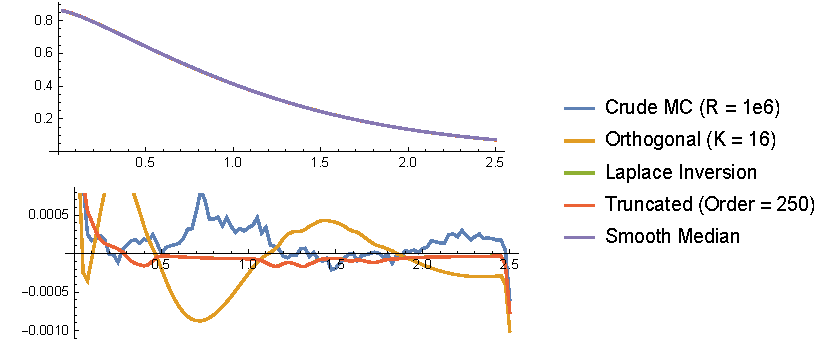
\includegraphics[width=0.95\textwidth]{poisson_gamma_svf.pdf}
\caption{Survival function estimates and approximate absolute error.}
\end{figure}

\begin{figure}[H]
\centering
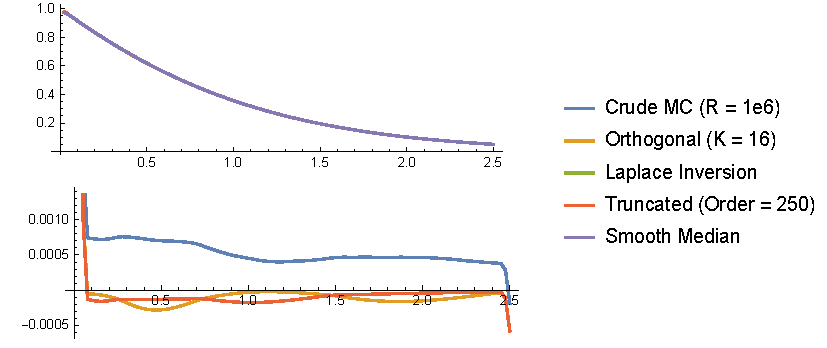
\includegraphics[width=0.95\textwidth]{poisson_gamma_slp.pdf}
\caption{Stop-loss premium estimates and approximate absolute error.}
\end{figure}


\begin{test}
$N\sim\PascalDist(\alpha=10,p=1/6)$, and $U\sim\GammaDist(r=3/2,m=1/75)$
\end{test}

This test case (up to the scaling constant) has been considered by Jin et al.\ \cite[Example 3]{JiPrRe16}. In the plots for this test case, the orthogonal estimator, the Laplace inversion estimator, and the truncated estimator all give the same values and hence are hidden underneath the red line for the truncated estimator.

\begin{figure}[H]
\centering
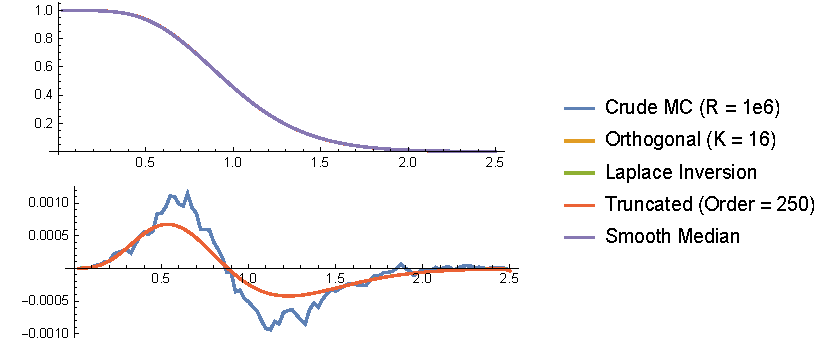
\includegraphics[width=0.95\textwidth]{pascal_gamma_svf.pdf}
\caption{Survival function estimates and approximate absolute error.}
\end{figure}

\begin{figure}[H]
\centering
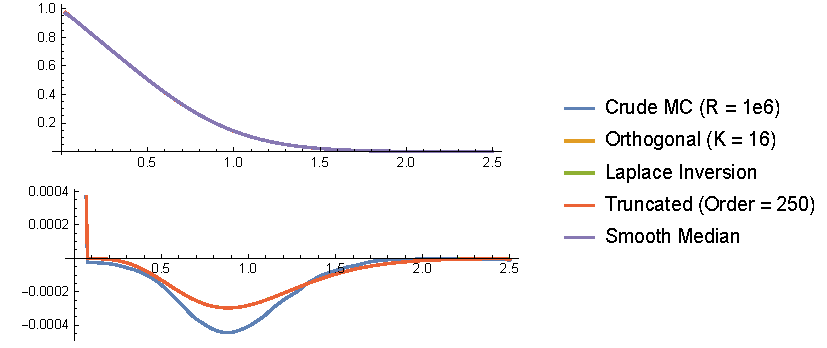
\includegraphics[width=0.95\textwidth]{pascal_gamma_slp.pdf}
\caption{Stop-loss premium estimates and approximate absolute error.}
\end{figure}

\begin{test} \label{test:poiss_pareto} $N\sim\PoissonDist(\lambda=4)$, and $U\sim\ParetoDist(a=5,b=11,\theta=0)$
\end{test}
The Laplace inversion estimator breaks down for small values of $x$ or $a$ in this test case. The specific error given is an ``out of memory'' exception when \textsc{Mathematica} is attempting to do some algebra with extremely large numbers. It is unclear whether a different implementation or selection of parameters would fix this behaviour.

\begin{figure}[H]
\centering
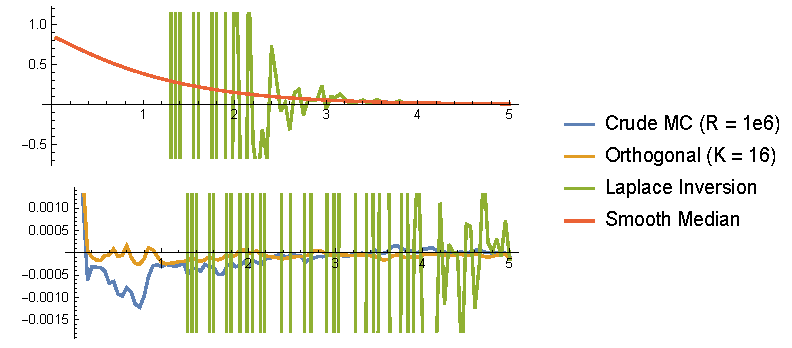
\includegraphics[width=0.95\textwidth]{poisson_pareto_svf.pdf}
\caption{Survival function estimates and approximate absolute error.}
\end{figure}

\begin{figure}[H]
\centering
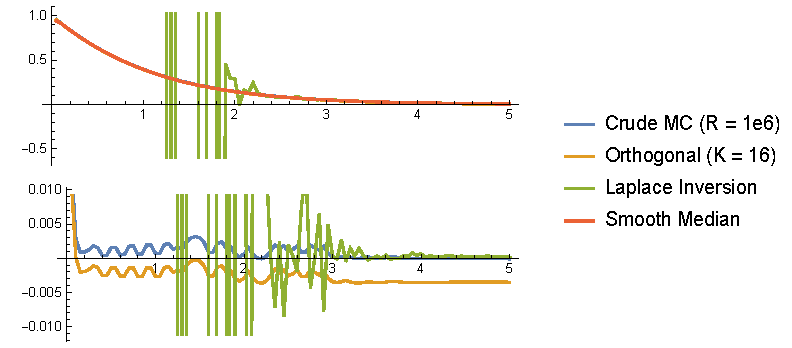
\includegraphics[width=0.95\textwidth]{poisson_pareto_slp.pdf}
\caption{Stop-loss premium estimates and approximate absolute error.}
\end{figure}

\begin{test} $N \sim \PascalDist(\alpha=2,p=1/4)$, and $U \sim \WeibullDist(\beta=1/2,\lambda=1/2)$
\end{test}

\begin{figure}[H]
\centering
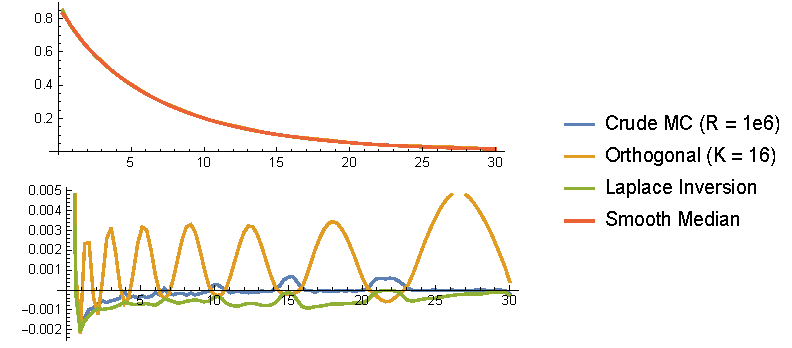
\includegraphics[width=0.95\textwidth]{pascal_weibull_svf.pdf}
\caption{Survival function estimates and approximate absolute error.}
\end{figure}

\begin{figure}[H]
\centering
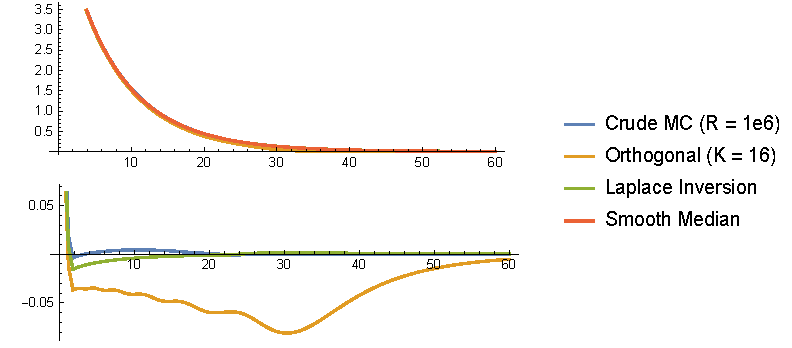
\includegraphics[width=0.95\textwidth]{pascal_weibull_slp.pdf}
\caption{Stop-loss premium estimates and approximate absolute error.}
\end{figure}


\subsection{Finite-time ruin probability with no initial reserve} \label{subsec:ApproximationFiniteTimeRuinProbability}

The plots above have used common random numbers to smooth the estimators, however this isn't possible in the following plots so they will appear less smooth.

\begin{test}
$\lambda=4$ and $U\sim\GammaDist(r=2,m=2)$ and $c=1$
\end{test}


\begin{figure}[H]
\centering
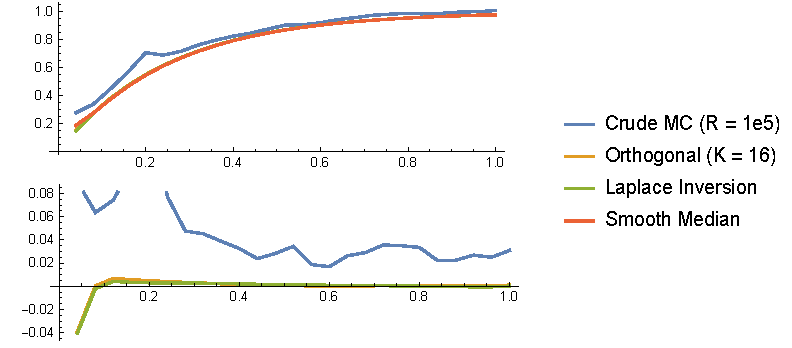
\includegraphics[width=0.95\textwidth]{poisson_exponential_ruin.pdf}
\caption{Ruin probability $\psi(0, t)$ estimates and approximate absolute error.}
\end{figure}


\begin{test} $\lambda=2$ and $U \sim \ParetoDist(a=5,b=11,\theta=0)$ and $c=1$
\end{test}

See the discussion of Test~\ref{test:poiss_pareto} for a description of the Laplace inversion estimator's poor behaviour when Pareto variables are involved.

\begin{figure}[H]
\centering
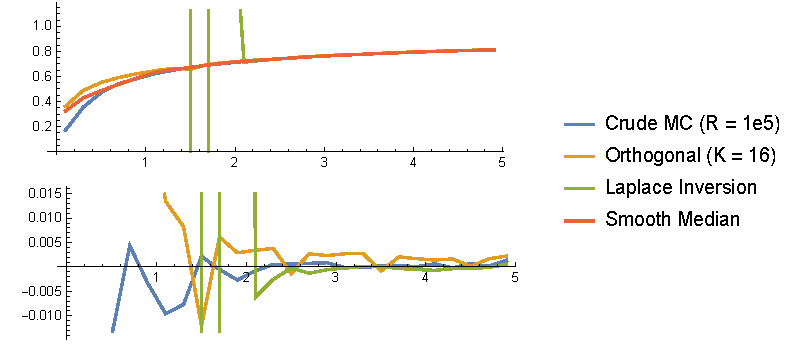
\includegraphics[width=0.95\textwidth]{poisson_pareto_ruin.pdf}
\caption{Ruin probability $\psi(0, t)$ estimates and approximate absolute error.}
\end{figure}
\subsection{Concluding remarks}
The orthogonal polynomial method has performed well across all the test cases studied. The accuracy is acceptable even with a rather small order of truncation $K=16$. It produces an approximation having an analytical expression, which is desirable, and in a timely manner. The precision may be improved by adding more terms in the expansions. The main drawback is probably the need for a parametrisation tailored to the case studied.

The Laplace transform inversion method yields outstanding result in terms of accuracy. It failed to provide a stable approximation for Pareto distributed claim sizes. The parametrisation is automatic and seems to fit the different case studied (except the Pareto one).

The main conclusion is that both methods are easy to implement and are superior to a simple truncation or a crude Monte Carlo approach.